% IEEE standard conference template; to be used with:
%   spconf.sty  - LaTeX style file, and
%   IEEEbib.bst - IEEE bibliography style file.
% --------------------------------------------------------------------------

\documentclass[letterpaper]{article}
\usepackage{spconf,amsmath,amssymb,graphicx}
\usepackage[hidelinks]{hyperref}

\usepackage{subcaption}
\usepackage{tikz}
\usetikzlibrary{arrows.meta}
\usetikzlibrary{positioning}
\usetikzlibrary{arrows}

% Example definitions.
% --------------------
% nice symbols for real and complex numbers
\newcommand{\R}[0]{\mathbb{R}}
\newcommand{\C}[0]{\mathbb{C}}

% bold paragraph titles
\newcommand{\mypar}[1]{{\bf #1.}}

% Title.
% ------
\title{Efficient Parallelization of Bor\r{u}vka's Minimum Spanning Tree Algorithm}

% Single address.
% ---------------
%\name{Matteo Kamm, Hulda Lilja Hannesdóttir, Mike Marti, Samuel Anzalone, Simon Hrabec} 
%\address{Computer Science Master, Computational Science Bachelor\\ ETH Z\"urich\\Z\"urich, Switzerland}


% Five authors (custom command).
% ----------------------------------------------------------
\fiveauthors
  {Samuel Anzalone \\[-0.8ex] {\small BS Computational Science} \\[-0.8ex] {\small \texttt{ansamuel@ethz.ch}}}
  {Mike Marti \\[-0.8ex] {\small MS Computer Science} \\[-0.8ex] {\small \texttt{mikmarti@ethz.ch}}}
  {Matteo Kamm \\[-0.8ex] {\small MS Computer Science} \\[-0.8ex] {\small \texttt{matkamm@ethz.ch}}}
  {Hulda L.\ Hannesdóttir \\[-0.8ex] {\small MS Computer Science} \\[-0.8ex] {\small \texttt{hhannesdo@ethz.ch}}}
  {\v{S}imon Hrabec \\[-0.8ex] {\small MS Computer Science} \\[-0.8ex] {\small \texttt{shrabec@ethz.ch}}}

\begin{document}
%\ninept
%
\maketitle
%

The hard page limit is 6 pages in this style. Do not reduce font size
or use other tricks to squeeze. This pdf is formatted in the American letter format, so the spacing may look a bit strange when printed out.

\begin{abstract}
Describe in concise words what you do, why you do it (not necessarily
in this order), and the main result.  The abstract has to be
self-contained and readable for a person in the general area. You
should write the abstract last.
\end{abstract}

\section{Introduction}
\label{sec:intro}
In this section we briefly introduce and explain what Minimum-Spanning-Tree algorithms can be used for. In addition, we
will go into more detail about our contribution to the scientific comunity as well as present work related to ours.

\mypar{Motivation}
Minimum-Spanning-Tree (MST) algorithms are used to compute a spanning tree of a given graph with edge weights. The goal
of the algorithm is to minimize the sum of all edge weights of the computed spanning tree.

The MST problem is one of the most studied problems in combinatorial optimization \cite{graham1985history}. Though its
solution is rather simple, it can often be used as part of other algorithms to compute intermediate results and is also
applicable in other scientific fields, such as medicine. Examples of problems that can be solved using MST algorithms
include
\begin{itemize}
  \item \textbf{Networking} MST algorithms can be used to find efficient solutions for the Spanning Tree Protocol, which
    is used to avoid looping of packages on the network layer.
  \item \textbf{$\frac{3}{2}$-ap\-prox\-i\-mate metric TSP} By combining algorithms that solve the eulertour, minimum
    matching and MST problem, one can develop a $\frac{3}{2}$-ap\-prox\-i\-mate algorithm solving the metric traveling
    salesperson problem \cite{christofides1976worst}.
  % TODO This sentance is copied from one of the cited abstracts. Is that ok?
  \item \textbf{Molecular Epidemiology} Minimum-Spanning-Trees are used in molecular epidemiology research to estimate
    relationships among individual strains or isolates \cite{spada2004use, salipante2011inadequacies}.
  \item \textbf{Machine Learning} MSTs can be used in machine learning environments. For example, MSTs can be used to
    reduce the fraction of incorrectly labeled samples when performing brain MRI tissue classification
    \cite{cocosco2003fully}.
\end{itemize}
For most of these use cases, the speed of the MST algorithm is of utmost importance to e.g. get quick medical results
and be able to treat the patient accordingly.

\mypar{Contribution}
In our research, we focused on the MST algorithm proposed by Bor\r{u}vka \cite{boruuvka1926jistem,
nevsetvril2001otakar}, which is one of the most prominent MST algorithms as of today. We implemented this algorithm
using different implementation and work distribution strategies. Our implementations use the Message Passing Interface
(MPI) protocol for work distribution and communication. To test the performance of our implementations, we use a seeded
randomized Kronecker graph generator.
% TODO This is not good :(. All other research talkes about how the MST is constructed.
As a limitation, our implementations don't store and return the MST itself, but only the total weight of it.

\mypar{Related Work}
% TODO maybe find more references for the first paragraph
As the MST problem is very versitile and can be used in various scientific disciplines, there has already been some
research into the parallelization capabilities of MST algorithms. One such paper \cite{chung1996parallel}, which is also
the main inspriation of this research project, looks into how the performance of Bor\r{u}vka behaves when using
different pointer jumping schemes. In addition, this paper introduces the randomized linear work Supervertex Pointer
Jumping scheme.

Other research focuses on the difference in performance with regards to the used computation model
\cite{dehne1998practical} and there has also been research conducted on the parallelization capabilities of the MST
problem using GPUs \cite{de2017parallel}.

Our research is similar to that of Chung and Condon \cite{chung1996parallel}, but differs in that we also look at
different work distribution strategies.

% TODO remove
% Do not start the introduction with the abstract or a slightly modified
% version. It follows a possible structure of the introduction. 
% Note that the structure can be modified, but the
% content should be the same. Introduction and abstract should fill at most the first page, better less.
%
% \mypar{Motivation} The first task is to motivate what you do.  You can
% start general and zoom in one the specific problem you consider.  In
% the process you should have explained to the reader: what you are doing,
% why you are doing, why it is important (order is usually reversed).
%
% For example, if my result is the fastest sorting implementation ever, one
% could roughly go as follows. First explain why sorting is important
% (used everywhere with a few examples) and why performance matters (large datasets,
% realtime). Then explain that fast implementations are very hard and
% expensive to get (memory hierarchy, vector, parallel). 
%
% Now you state what you do in this paper. In our example: 
% presenting a sorting implementation that is
% faster for some sizes as all the other ones.
%
% \mypar{Related work} Next, you have to give a brief overview of
% related work. For a report like this, anywhere between 2 and 8
% references. Briefly explain what they do. In the end contrast to what
% you do to make now precisely clear what your contribution is.

\section{Background}
\label{sec:background}
In this section we will introduce the MST problem itself, as well as Bor\r{u}vka's algorithm and different
parallelization strategies used in our implementations.

\mypar{Spanning Tree/Forest}
TODO

\mypar{Minimum-Spanning-Tree Problem}
TODO

\mypar{Bor\r{u}vka's Algorithm}
TODO

\mypar{Union Find Datastructure}
TODO

\mypar{Pointer Jumping}
TODO

\mypar{Supervertex Pointer Jumping}
TODO

\mypar{MPI}
TODO

\mypar{Kronecker Graphs}
% TODO Not sure if this is the original paper that introduced kronecker graphs (double check)
TODO \cite{leskovec2010kronecker}

% Give a short, self-contained summary of necessary
% background information. For example, assume you present an
% implementation of sorting algorithms. You could organize into sorting
% definition, algorithms considered, and asymptotic runtime statements. The goal of the
% background section is to make the paper self-contained for an audience
% as large as possible. As in every section
% you start with a very brief overview of the section. Here it could be as follows: In this section 
% we formally define the sorting problem we consider and introduce the algorithms we use
% including a cost analysis.
%
% \mypar{Sorting}
% Precisely define sorting problem you consider.
%
% \mypar{Sorting algorithms}
% Explain the algorithm you use including their costs.
%
% As an aside, don't talk about "the complexity of the algorithm.'' It's incorrect,
% problems have a complexity, not algorithms.


\section{Approach}
\label{sec:approach}
% Now comes the ``beef'' of the report, where you explain what you
% did. Again, organize it in paragraphs with titles. As in every section
% you start with a very brief overview of the section.

% In this section, structure is very important so one can follow the technical content.

% Mention and cite any external resources that you used including libraries or other code.

% TODO if the space allows for it, use subsections instead of only paragraphs
This section contains information about the different implementations that we developed, as well as other technical
details, such as distribution strategies, limitations and the benchmarking infrastructure.

\subsection{Distributing the Work}
There are many ways as to how a graph can be distributed among multiple computation units. The two strategies that we
looked into are distributing the work by edges, including their endpoint information, and distributing the work by
vertices, including their incident edges. A combination of the two would also be possible, but was not considered in
this project. As these two strategies have vastly different parallelization capabilities, we developed multiple
implementations for both of these approaches. To get a better understanding of how they work, as well as their
advantages and disadvantages, we describe them both in the following two paragraphs.

% TODO maybe move the original input graph into the middle to clearly separate the edge dist. and vertex dist. images
\begin{figure*}
  \begin{subfigure}{0.33\textwidth}
    \centering
    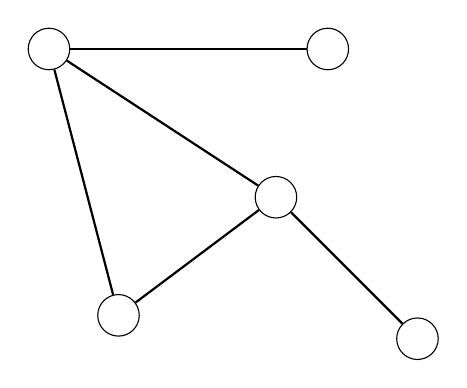
\begin{tikzpicture}[every node/.style={circle,draw,align=center,font=\small,minimum size=1.5em},
      node distance=3cm]
      \node (v1) {};
      \node[below right=3cm and .5cm of v1] (v2) {};
      \node[below right=1.5cm and 2.5cm of v1] (v3) {};
      \node[below right=2cm of v3] (v4) {};
      \node[right=of v1] (v5) {};
      \path[>={Stealth[black]}, every edge/.style={draw=black, thick}]
        (v1) edge (v2)
        (v1) edge (v3)
        (v1) edge (v5)
        (v2) edge (v3)
        (v3) edge (v4);
    \end{tikzpicture}
    \caption{Original input graph.}
    \label{fig:work_distribution_original_input_graph}
  \end{subfigure}
  \begin{subfigure}{0.33\textwidth}
    \centering
    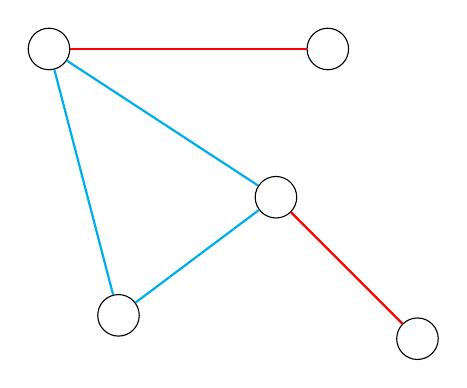
\begin{tikzpicture}[every node/.style={circle,draw,align=center,font=\small,minimum size=1.5em},
      node distance=3cm]
      \node (v1) {};
      \node[below right=3cm and .5cm of v1] (v2) {};
      \node[below right=1.5cm and 2.5cm of v1] (v3) {};
      \node[below right=2cm of v3] (v4) {};
      \node[right=of v1] (v5) {};
      \path[>={Stealth[black]}, every edge/.style={draw=black, thick}]
        (v1) edge[cyan] (v2)
        (v1) edge[cyan] (v3)
        (v1) edge[red] (v5)
        (v2) edge[cyan] (v3)
        (v3) edge[red] (v4);
    \end{tikzpicture}
    \caption{Edge distributed input graph.}
    \label{fig:work_distribution_edge_distributed_graph}
  \end{subfigure}
  \begin{subfigure}{0.33\textwidth}
    \centering
    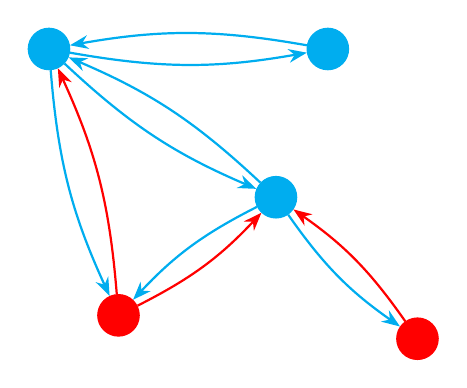
\begin{tikzpicture}[every node/.style={circle,draw,align=center,font=\small,minimum size=1.5em},
      node distance=3cm]
      \node[cyan, fill=cyan] (v1) {};
      \node[red, fill=red, below right=3cm and .5cm of v1] (v2) {};
      \node[cyan, fill=cyan, below right=1.5cm and 2.5cm of v1] (v3) {};
      \node[red, fill=red, below right=2cm of v3] (v4) {};
      \node[cyan, fill=cyan, right=of v1] (v5) {};
      \path[>={Stealth[black]}, every edge/.style={draw=black, thick}]
        [->] [>={Stealth[cyan]}] (v1) edge[cyan, bend right=10] (v2)
        [->] [>={Stealth[red]}] (v2) edge[red, bend right=10] (v1)
        [->] [>={Stealth[cyan]}] (v1) edge[cyan, bend right=10] (v3)
        [->] [>={Stealth[cyan]}] (v3) edge[cyan, bend right=10] (v1)
        [->] [>={Stealth[cyan]}] (v1) edge[cyan, bend right=10] (v5)
        [->] [>={Stealth[cyan]}] (v5) edge[cyan, bend right=10] (v1)
        [->] [>={Stealth[red]}] (v2) edge[red, bend right=10] (v3)
        [->] [>={Stealth[cyan]}] (v3) edge[cyan, bend right=10] (v2)
        [->] [>={Stealth[cyan]}] (v3) edge[cyan, bend right=10] (v4)
        [->] [>={Stealth[red]}] (v4) edge[red, bend right=10] (v3);
    \end{tikzpicture}
    \caption{Vertex distributed input graph.}
    \label{fig:work_distribution_vertex_distributed_graph}
  \end{subfigure}
  \caption{Work distribution example.}
  \label{fig:work_distribution}
\end{figure*}

\mypar{Distribution by Edges}
In this approach, we distribute the edges of the input graph as evenly as possible among all available computation
units. An example of how such a distribution would look like can be seen in Fig.
\ref{fig:work_distribution_edge_distributed_graph}. This strategy allows for a very fair work distribution, as every
computation unit has approximately an equal amount of work during the selection of the minimum outgoing edge of every
component. On the other hand, the merging of components cannot be parallelized using this approach. This is because
during the process of merging all nodes inside a component have to agree on a unique component identifier, which is a
process performed on vertices, not edges.

\mypar{Distribution by Vertices}
In this approach, we distribute the vertices of the input graph, including their incident edges, as evenly as possible
among all available computation units. An example of how such a distribution would look like can be seen in Fig.
\ref{fig:work_distribution_vertex_distributed_graph}. A major disadvantage of this approach is that all edges have to be
distributed twice, as it is not guaranteed that the neighboring vertex gets distributed to the same computation unit. As
such, this strategy requires a lot more work to distribute the graph information. In addition, the work is not
distributed as fair as when using the edge distribution strategy, because a computation unit could end up with vertices
that have a lot of incident edges, whilst another computation unit could end up with vertices that have almost no
incident edges. As such, the computation of the minimum outgoing edge of every component is not as fair as it is in our
other strategy. However, in this approach the merging of components can easily be parallelized.

\subsection{Implementations}
We developed various implementations using C++17, combining different merging approaches with the two aformentioned
distribution strategies. Here is a list of all the combinations that we developed:
\begin{itemize}
  \item ... % TODO
\end{itemize}
As one can see, this list does not contain every possible combination. This is because after some intermediate
benchmarking we focussed on the strategies that were the most promissing, namely union find and edge distribution.
% TODO explain edge removal implementation
We also implemented sequential versions for some of the merging strategies, to get a better understanding of them.
However, these sequential algorithms did not serve any additional purpose beyond that, i.e. they were not used to get
any measurements.

\mypar{Baseline Implementation}
To get an idea of how well our implementations perform, we decided to use parallel Boost as our baseline. This shows us
how well our implementations hold up against current industry standard code. The reason why we chose parallel Boost is
because it is considered to be the de facto standard when it comes to parallel graph libraries for C++.

\mypar{Kronecker Graph Generator}
We first experimented with different graph types and even implemented some generators for them, but ultimately decided
to only use kronecker graphs, as ... % TODO reason why kronecker graphs are used for such tests
The generator implementation that we used is the official graph500 open source version available on
GitHub\footnote{\url{https://github.com/graph500/graph500/tree/newreference/generator}}, which we copied into our
project and call directly from the source. To get fair and comparable benchmarking results, we seeded the graph
generator, such that it always generated the same random graph, no matter the algorithm that gets executed.

\mypar{Communication}
% TODO mention how mpi was used

\mypar{Limitations}
So far all implementations don't compute the actual MST, but only its edge weight sum. All the heavy lifting is done anyway since in every iteration in our fastest implementation, all computation units know which edges were added to the MST. In addition, the work has to be distributed among all computation units evenly, i.e. the amount of edges or vertices must be divisible by the amount of
computation units depending on whether it is an edge or vertex distributed algorithm. Though in most implementations
both of these limitations would be quite easy to implement, we disregarded them as being low priority, as our focus lied
on the difference between the various implementation strategies.
% TODO maybe add that it only works with ints so far

\mypar{Correctness}
The correctness of the implementation comes down to the fact that all implementations only terminate once no new edge is
selected, by any computation unit, to the resulting MST. For that reason, the result is a spanning tree. The computed
spanning tree is also a MST due to the greedy nature of how they're chosen. The same proof holds as for why the
Bor\r{u}vka's algorithm is correct\cite{nevsetvril2012origins}. For verifying the correctness we use unit tests. We
wrote multiple manual unit tests that cover different edge cases to ensure the correctness of our implementations. On
top of that we also use differential testing with larger Kronocker Graphs (1024 vertices), using the result of the
parallel Boost implementation as a comparison. To get assurance during development and be able to more quickly merge
open pull requests, used continuous integration to build the application and execute the available unit tests.

\subsection{Benchmarking Infrastructure}
% TODO maybe move likwid description to background
To make the experimentation process faster, we developed a small benchmarking infrastructure that allows us to more
easily benchmark the various algorithms with different graph sizes. The measurements were performed using the
performance measurement tool LIKWID \cite{treibig2010likwid}. LIKWID uses hardware counters for its measurements and can
be invoked by putting markers around the code that should be benchmarked. This allowed us to not only benchmark the
entire execution, but also individual parts of the algorithms, which gave us more detailed information about which parts
require the most amount of work.

\section{Experimental Results}\label{sec:exp}

Here you evaluate your work using experiments. You start again with a
very short summary of the section. The typical structure follows.

\mypar{Experimental setup} Specify the platform (processor, frequency, maybe OS, maybe cache sizes)
as well as the compiler, version, and flags used. If your work is about performance, 
I strongly recommend that you play with optimization flags and consider also icc for additional potential speedup.

Then explain what kind of benchmarks you ran. The idea is to give enough information so the experiments are reproducible by somebody else on his or her code.
For sorting you would talk about the input sizes. For a tool that performs NUMA optimization, you would specify the programs you ran.

\mypar{Results}
% TODO compare to results from Chung and Condon
Next divide the experiments into classes, one paragraph for each. In each class of experiments you typically pursue one questions that then is answered by a suitable plot or plots. For example, first you may want to investigate the performance behavior with changing input size, then how your code compares to external benchmarks.

For some tips on benchmarking including how to create a decent viewgraph see pages 22--27 in \cite{Pueschel:10}.

{\bf Comments:}
\begin{itemize}
\item Create very readable, attractive plots (do 1 column, not 2 column plots
for this report) with readable font size. However, the font size should also not be too large; typically it is smaller than the text font size.
An example is in Fig.~\ref{fftperf} (of course you can have a different style).
\item Every plot answers a question. You state this question and extract the
answer from the plot in its discussion.
\item Every plot should be referenced and discussed.
\end{itemize}

\begin{figure}\centering
  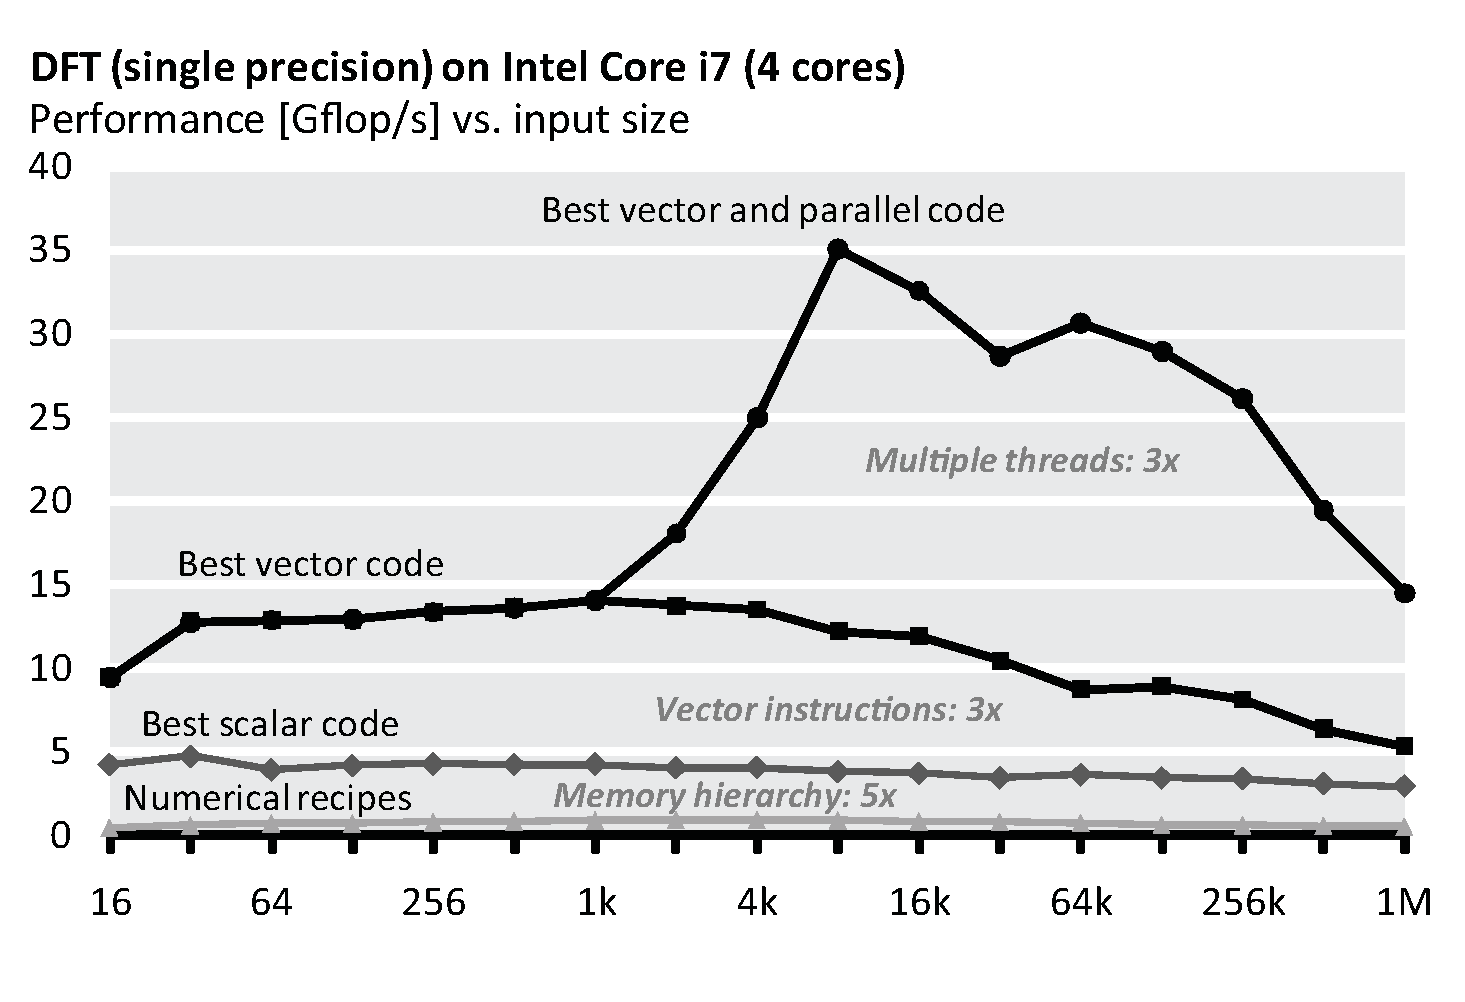
\includegraphics[scale=0.33]{dft-performance.eps}
  \caption{Performance of four single precision implementations of the
  discrete Fourier transform. The operations count is roughly the
  same. The labels in this plot are maybe a little bit too small.\label{fftperf}}
\end{figure}

\section{Conclusions}

Here you need to summarize what you did and why this is
important. {\em Do not take the abstract} and put it in the past
tense. Remember, now the reader has (hopefully) read the report, so it
is a very different situation from the abstract. Try to highlight
important results and say the things you really want to get across
such as high-level statements (e.g., we believe that .... is the right
approach to .... Even though we only considered x, the
.... technique should be applicable ....) You can also formulate next
steps if you want. Be brief. After the conclusions there are only the references.

\section{Further comments}

Here we provide some further tips.

\mypar{Further general guidelines}

\begin{itemize}
\item For short papers, to save space, I use paragraph titles instead of
subsections, as shown in the introduction.

\item It is generally a good idea to break sections into such smaller
units for readability and since it helps you to (visually) structure the story.

\item The above section titles should be adapted to more precisely
reflect what you do.

\item Each section should be started with a very
short summary of what the reader can expect in this section. Nothing
more awkward as when the story starts and one does not know what the
direction is or the goal.

\item Make sure you define every acronym you use, no matter how
convinced you are the reader knows it.

\item Always spell-check before you submit (to us in this case).

\item Be picky. When writing a paper you should always strive for very
high quality. Many people may read it and the quality makes a big difference.
In this class, the quality is part of the grade.

\item Books helping you to write better: \cite{Higham:98} and \cite{Strunk:00}.

\item Conversion to pdf (latex users only): 

dvips -o conference.ps -t letter -Ppdf -G0 conference.dvi

and then

ps2pdf conference.ps
\end{itemize}

\mypar{Graphics} For plots that are not images {\em never} generate the bitmap formats
jpeg, gif, bmp, tif. Use eps, which means encapsulate postscript. It is
scalable since it is a vector graphic description of your graph. E.g.,
from Matlab, you can export to eps.

The format pdf is also fine for plots (you need pdflatex then), but only if the plot was never before in the format 
jpeg, gif, bmp, tif.


% References should be produced using the bibtex program from suitable
% BiBTeX files (here: bibl_conf). The IEEEbib.bst bibliography
% style file from IEEE produces unsorted bibliography list.
% -------------------------------------------------------------------------
\bibliographystyle{IEEEbib}
\bibliography{bibl_conf}

\end{document}

